\documentclass[runningheads]{llncs}

\usepackage[T1]{fontenc}
\usepackage[utf8]{inputenc}
\usepackage{graphicx}
\usepackage{amssymb}
\usepackage{booktabs}
\usepackage{hyperref}
\usepackage{enumitem}
\usepackage{float}

% Encontrar figuras quer se compile a partir de docs/ quer da raiz do repo
\graphicspath{{../results/}{../results/figures/}{results/}{results/figures/}}

\providecommand{\doi}[1]{\url{https://doi.org/#1}}

\renewcommand\UrlFont{\color{blue}\rmfamily}
\urlstyle{rm}

\begin{document}
\sloppy

\title{Navegação Autónoma na Formula Student: Uma Abordagem Baseada em Aprendizagem por Reforço}
\titlerunning{Navegação Autónoma na Formula Student com RL}

\author{Luís Miguel Pereira Silva \and
Pedro Miguel S.\ A.\ Urbano dos Reis}

\authorrunning{L. Silva e P. Reis}

\institute{Mestrado em Inteligência Artificial, Universidade do Minho, Braga, Portugal\\
\email{\{pg60390,pg59908\}@alunos.uminho.pt}}

\maketitle

\begin{abstract}
Este relatório apresenta um sistema de condução autónoma para a categoria \textit{Driverless} da Formula Student, treinado de raiz com aprendizagem por reforço (RL). Foi desenvolvido um ambiente de simulação 2D, compatível com a API \textit{Gymnasium}, que integra um modelo cinemático de bicicleta, um sensor de cones com ruído realista, 14 traçados oficiais de competição em formato YAML e as regras FS-AI (penalizações por cone, \textit{Down-Or-Out}, \textit{off-course} gradual). O agente principal é um \textit{Soft Actor-Critic} (SAC), comparado com \textit{Proximal Policy Optimization} (PPO) como \textit{baseline}, treinado com \textit{domain randomization} e avaliado sob um \textit{split} canónico de 9 pistas de treino e 5 inéditas de teste. O SAC apresenta um \textit{lap rate} comparável ao PPO (66\% vs.\ 68\%) mas é cerca de duas vezes mais seguro (2.4 vs.\ 4.8 cones derrubados). Identificámos, via pistas espelhadas, um \textbf{viés direcional} sistemático ($-25$\,pp, invisível ao \textit{split} de teste tradicional) e uma assimetria de robustez de perceção: a política tolera falhas transientes do sensor mas colapsa com cones fisicamente em falta. Ambas as fraquezas se corrigem com \textit{data augmentation} dirigida (\textit{mirror} e \textit{cone-dropout}), cuja combinação é super-aditiva e sem custo no desempenho base. Quinze ablações e um estudo iterativo de \textit{reward shaping} quantificam a contribuição de cada componente.
\keywords{Aprendizagem por Reforço \and Condução Autónoma \and Formula Student \and Soft Actor-Critic \and Generalização \and Domain Randomization}
\end{abstract}

% =====================================================================
\section{Introdução e Definição do Problema}
% =====================================================================

A Formula Student é a maior competição de engenharia automóvel universitária a nível mundial. A categoria \textit{Driverless} desafia as equipas a desenvolver veículos totalmente autónomos, capazes de navegar numa pista delimitada por cones coloridos --- azuis (fronteira esquerda), amarelos (fronteira direita) e laranja (linha de partida/chegada) --- sem qualquer intervenção humana~\cite{kabzan2020}. O veículo deve detetar cones, planear a trajetória e executar comandos de direção e aceleração em tempo real, completando a volta o mais depressa possível e sem derrubar cones (cada cone derrubado acrescenta uma penalização de tempo).

A abordagem clássica decompõe o problema num \textit{pipeline} de perceção, mapeamento, planeamento e controlo. Neste trabalho exploramos uma alternativa \textit{end-to-end} baseada em aprendizagem por reforço~\cite{sutton2018}: treinar um agente que aprenda a conduzir diretamente da sua perceção local, maximizando o progresso ao longo da pista e minimizando penalizações. O agente \textbf{não} tem acesso ao traçado global nem à \textit{centerline} ideal --- toda a informação de pista provém da observação dos cones, replicando o cenário \textit{onboard} real.

\paragraph{Estado da arte.} Os sistemas de competição estabelecidos, como o AMZ Driverless~\cite{kabzan2020}, seguem o \textit{pipeline} modular clássico (SLAM com cones, planeamento, controlo MPC), que exige engenharia extensa de cada módulo. Em paralelo, o RL \textit{end-to-end} tem produzido políticas competitivas em simuladores de corrida, dominantemente com SAC~\cite{haarnoja2018} e PPO~\cite{schulman2017} (implementações de referência no Stable-Baselines3~\cite{raffin2021}), incluindo aplicações recentes à Formula Student Driverless~\cite{ulrich2024}; a transferência para fora da distribuição de treino apoia-se em \textit{domain randomization}~\cite{tobin2017} e \textit{data augmentation}. A literatura avalia quase sempre em pistas inéditas, mas raramente sonda eixos de generalização estruturais (direção das curvas, densidade de cones) --- o foco da nossa avaliação.

Este relatório documenta a solução implementada e os resultados obtidos. As contribuições principais são: (i)~um ambiente de simulação FS-AI 2D, leve e reprodutível, com 14 pistas reais de competição; (ii)~uma comparação multi-\textit{seed} entre SAC e PPO sob um protocolo de generalização rigoroso; (iii)~a identificação e correção de um viés direcional estrutural, normalmente mascarado pelos \textit{splits} de teste convencionais; (iv)~uma análise de robustez de perceção que distingue falhas transientes de cones em falta, corrigida com \textit{augmentation} dirigida; e (v)~um conjunto de 15 ablações e um estudo iterativo de \textit{reward shaping} que isolam o contributo de cada decisão de \textit{design}. O código encontra-se em \url{https://github.com/pedroreis2468/AR2}; o notebook de avaliação executável (\texttt{notebooks/overview.ipynb}) reproduz todas as tabelas e figuras deste relatório.

% =====================================================================
\section{Ambiente de Simulação}
% =====================================================================

O treino é conduzido inteiramente em simulação, num ambiente desenvolvido de raiz que segue a API \textit{Gymnasium} (\texttt{FSRacingEnv}). A simulação opera a 50\,Hz com \textit{action repeat} de 2, pelo que o agente decide a 25\,Hz.

\paragraph{Modelo do veículo.} Utilizámos um modelo cinemático de bicicleta~\cite{kong2015} referenciado ao centro de gravidade, calibrado para um carro FS típico ($\sim$250\,kg, \textit{wheelbase} de 1.55\,m, $\mu = 1.5$). O modelo inclui \textit{rate limiting} no \textit{steering} ($\dot{\delta}_{\max}=1.5$\,rad/s) e uma restrição de \textit{friction circle}, $a_\mathrm{lat}^2 + a_\mathrm{lon}^2 \leq (\mu g)^2$, que limita a aceleração combinada e penaliza implicitamente o excesso de velocidade em curva.

\paragraph{Pistas: reais e procedurais.} O sistema suporta duas fontes de pistas. (i)~\textbf{Pistas reais de competição}: 14 traçados oficiais FS em formato YAML, obtidos do projeto PacSim (FSG19/21/23/24, FSE22 ($\times$2)/23/24, FSI24, FSCZ24, FSO20, FSS19, FSS22 V1/V2), carregados por um \texttt{YAMLTrackLoader} e suavizados com \textit{splines} cúbicas periódicas. (ii)~\textbf{Geração procedural}: pontos de controlo numa elipse perturbada, suavizados com \textit{splines} fechadas e re-amostrados a cada episódio --- usados como \textit{fallback} e para aumentar a diversidade.

\paragraph{Perceção.} Um sensor de cones (FOV de $180^\circ$, alcance de 15\,m) devolve os 3 cones mais próximos de cada cor no referencial do carro, com ruído gaussiano na distância ($\sigma=0.2$\,m) e no \textit{bearing} ($\sigma=0.007$\,rad) e probabilidade de deteção de 95\%, emulando uma \textit{pipeline} de visão YOLO + \textit{stereo depth}. Cones derrubados são \textbf{removidos persistentemente} do FOV, refletindo o seu impacto na perceção real.

\paragraph{Regras FS-AI e colisão.} A deteção de colisão usa uma \textit{bounding box} retangular do veículo. Cada cone azul/amarelo derrubado custa +2\,s (penalização de tempo) e os cones laranja custam o dobro. A terminação do episódio (\textit{Down-Or-Out}, DOO) ocorre quando: (a)~$\geq$10 cones são derrubados; (b)~o desvio lateral à \textit{centerline} excede 5\,m; ou (c)~o veículo permanece \textit{off-course} mais de 2\,s consecutivos. Detetam-se também situações de contramão e de estagnação (progresso $<$2\,m em 300 \textit{steps}).

% =====================================================================
\section{Metodologia}
% =====================================================================

O problema é formulado como um processo de decisão de Markov (MDP) com $\gamma = 0.99$.

\paragraph{Observação ($\mathbf{s} \in \mathbb{R}^{24}$).} 6 dimensões de estado do veículo ($v_x$, $v_y$, $\omega$, $\delta$, $a_x$, $a_y$, normalizadas) e 18 dimensões com as posições relativas $(x,y)$ dos 3 cones mais próximos de cada cor (azul, amarelo, laranja). Sublinhe-se que o agente \emph{não} recebe a \textit{centerline} nem as distâncias às fronteiras: o planeamento global tem de emergir do comportamento reativo. A \textit{flag} \texttt{--legacy-obs} reduz a observação a 18 dimensões (sem cones laranja), para compatibilidade com modelos antigos.

\paragraph{Ação ($\mathbf{a} \in [-1,1]^2$).} \textit{Steering} normalizado e um comando unificado de \textit{throttle}/travão (negativo = travão).

\paragraph{Reward shaping.} A recompensa por \textit{step} combina os termos da Tabela~\ref{tab:reward}. O termo de progresso (com sinal, ao longo da \textit{centerline} ideal) é o sinal dominante; os restantes moldam um comportamento rápido, alinhado, suave e dentro da pista. Penalizações terminais ($-50$ para DOO, $-30$ para \textit{off-course timeout}, $-20$ para contramão) e um bónus de volta de $\max(200 - 5\,n_\mathrm{cones},\,50)$ calibram os comportamentos-limite. Esta configuração final resultou de um processo iterativo, documentado como estudo de \textit{design} na Secção~\ref{sec:reward_iter}.

\begin{table}[t]
\centering
\caption{Componentes da função de recompensa.}
\label{tab:reward}
\small
\begin{tabular}{llr}
\toprule
\textbf{Componente} & \textbf{Descrição} & \textbf{Peso} \\
\midrule
$r_\mathrm{progress}$ & Distância percorrida na \textit{centerline} (com sinal) & $\times 2.0$ \\
$r_\mathrm{alignment}$ & $v \cdot \cos(\theta_\mathrm{err})$ --- rápido \emph{e} alinhado & $\times 0.4$ \\
$r_\mathrm{smooth}$ & Penaliza $\Delta$\textit{steering} acima de \textit{dead-band} 0.1 & $\times 0.05$ \\
$r_\mathrm{lateral}$ & Linear dentro da pista, quadrática fora & $\times 0.08$ \\
$r_\mathrm{time}$ & Custo fixo por \textit{step} (encoraja velocidade) & $-0.005$ \\
\textit{cone hit} & Por cone azul/amarelo derrubado & $-8.0$ \\
\textit{orange hit} & Por cone laranja derrubado & $-16.0$ \\
\textit{lap bonus} & Por volta completa, descontado pelos cones & $+200$ \\
\bottomrule
\end{tabular}
\end{table}

\paragraph{Algoritmo principal: SAC.} O \textit{Soft Actor-Critic}~\cite{haarnoja2018} é um algoritmo \textit{off-policy} com maximização de entropia, adequado a controlo contínuo. Implementámos uma versão \textit{custom} em PyTorch (\textit{Gaussian actor} \textit{squashed}, \textit{twin Q-networks} MLP $256{\times}256$, \textit{target networks} com \textit{Polyak} $\tau{=}0.005$, \textit{replay buffer} de 1\,M e \textit{auto-tuning} da temperatura $\alpha$) para fins educativos, e usámos a implementação de produção do Stable-Baselines3~\cite{raffin2021} para os resultados reportados. A \textit{target entropy} foi fixada em $-0.5$ (em vez do \textit{default} $-\dim(\mathcal{A}){=}-2$) para evitar o colapso prematuro da exploração.

\paragraph{Baseline: PPO.} Como \textit{baseline} \textit{on-policy} usámos o PPO~\cite{schulman2017} (SB3), com a mesma arquitetura de rede ($256{\times}256$) para uma comparação justa.

\paragraph{Domain randomization.} Para promover robustez, cada episódio sorteia massa ($\pm 15\%$), atrito ($\pm 20\%$) e arrasto ($\pm 10\%$) do veículo, posição lateral e velocidade iniciais, e o ruído do sensor~\cite{tobin2017,ulrich2024}.

\paragraph{Data augmentation dirigida.} Em resposta às fraquezas estruturais identificadas nas Secções~\ref{sec:bias} e~\ref{sec:robustez}, introduzimos duas técnicas de \textit{augmentation} ao nível dos dados, sem alterar a função de recompensa: (i)~\textbf{mirror augmentation} --- com probabilidade 50\% a cada \textit{reset}, espelha a pista em Y (trocando cones azuis$\leftrightarrow$amarelos e recalculando tangentes/normais); (ii)~\textbf{cone-dropout augmentation} --- com probabilidade 50\% a cada \textit{reset}, remove uma fração uniforme em $[0,15\%]$ dos cones físicos, de forma persistente no episódio, mantendo a \textit{centerline} (e portanto a recompensa) intacta.

% =====================================================================
\section{Implementação e Protocolo Experimental}
% =====================================================================

\paragraph{Implementação e arquitetura de software.} O sistema (Python/PyTorch) organiza-se em quatro camadas: \texttt{env/} (ambiente \texttt{FSRacingEnv}: veículo, sensor, \textit{loader} YAML, gerador procedural, \textit{renderer} PyGame); \texttt{agent/} (SAC \textit{custom} educativo); \texttt{train.py}/\texttt{evaluate.py} (treino SB3 com 4--8 ambientes paralelos, avaliação com visualização); e \texttt{scripts/} (avaliação per-pista, agregação multi-\textit{seed}, figuras, espelhamento, \textit{sweeps} de robustez). Uma suite \texttt{pytest} (16 testes) cobre o contrato Gymnasium, o veículo e os \textit{splits}. Treino numa GPU RTX 5070\,Ti; avaliação em CPU. O notebook \texttt{notebooks/overview.ipynb}, entregue executado, reproduz os resultados e permite avaliação ao vivo.

\paragraph{Splits canónicos.} As 14 pistas de circuito são divididas num \textit{split} fixo de 9 pistas de treino (FSG19, FSG21, FSG23, FSE22, FSE22\_test, FSE23, FSO20, FSS19, FSS22\_V1) e 5 pistas de teste mantidas \textbf{completamente inéditas} durante o treino (FSG24, FSI24, FSCZ24, FSE24, FSS22\_V2). Como terceiro eixo de avaliação, geram-se as 14 versões \textbf{espelhadas em Y} (\textit{held-out}), que preservam a geometria mas invertem o sentido das curvas.

\paragraph{Modelos treinados.} SAC \textit{baseline} (3M \textit{steps}, 3 \textit{seeds}); PPO \textit{baseline} (6M \textit{steps}, 3 \textit{seeds}); 15 ablações de SAC (2M \textit{steps}, 1 \textit{seed} cada); e o \textit{design} factorial de \textit{augmentation} --- SAC + \textit{mirror}, SAC + \textit{cone-dropout} e SAC + ambas (3M \textit{steps}, 1 \textit{seed} cada).

\paragraph{Métricas.} \textit{Lap rate} (\% de episódios em que a volta é completada), número médio de cones derrubados, velocidade média e tempo de volta, agregados como $\bar{x}\pm\sigma$ entre \textit{seeds}.

\paragraph{Nota metodológica (avaliação estocástica).}
A avaliação per-track corre N=10 episódios por pista \textbf{com \textit{domain randomization} ativa}: os valores são \emph{estimativas da performance média sob variação}, não medições determinísticas, e re-execuções variam $\approx\pm5$--$8$\,pp no \textit{lap rate} (as fontes de aleatoriedade usam o gerador global do NumPy, não semeado pelo avaliador). Diferenças de poucos pontos percentuais estão portanto dentro do ruído amostral; os efeitos grandes (consistência SAC vs.\ PPO, viés direcional, efeito das \textit{augmentations}) situam-se muito acima dele.

% =====================================================================
\section{Resultados e Discussão}
% =====================================================================

\subsection{Engenharia iterativa da recompensa}
\label{sec:reward_iter}

Antes de qualquer comparação de algoritmos, o maior desafio prático foi obter uma recompensa que produzisse \emph{algum} comportamento útil: nas primeiras versões o carro mal se mexia ou não arriscava as curvas. Reconstruímos essa progressão, ancorada no histórico git (do \textit{commit} inicial \texttt{8c4cf3a} à recompensa de produção), como um \textbf{estudo de design de 6 iterações}, em que cada passo altera $\sim$um aspeto da recompensa e \textbf{todo o resto é mantido fixo} (algoritmo, pista, sensor, colisão, regras FS-AI). Cada iteração foi treinada até à convergência (SAC, 500\,k \textit{steps} $\times$ 3 \textit{seeds}). A Tabela~\ref{tab:reward_iter} resume a progressão e a Figura~\ref{fig:reward_iter} a sua evolução empírica.

\begin{table}[t]
\centering
\caption{Estudo de design da recompensa: 6 iterações, cada uma treinada até à convergência (SAC, 500\,k \textit{steps} $\times$ 3 \textit{seeds}). Métricas na pista de avaliação, $\bar{x}\pm\sigma$ entre \textit{seeds}.}
\label{tab:reward_iter}
\small
\begin{tabular}{clccc}
\toprule
\textbf{\#} & \textbf{Mudança na recompensa} & \textbf{Pista (\%)} & \textbf{Vel. (km/h)} & \textbf{Cones} \\
\midrule
1 & v0 ``suicide policy'': \textit{off-track} = morte instantânea & 76 $\pm$ 23 & 60 $\pm$ 22 & 2.7 \\
2 & \textit{Off-course} gradual (substitui a morte instantânea) & 83 $\pm$ 30 & 49 $\pm$ 26 & 3.4 \\
3 & Suavidade $-0.3\,|\Delta\delta|$ $\rightarrow$ $-0.05$ com \textit{dead-band} 0.1 & 100 $\pm$ 0 & 74 $\pm$ 7 & 4.0 \\
4 & Lateral quad.\ $\times 0.2$ $\rightarrow$ \textit{piecewise} $\times 0.08$ & 100 $\pm$ 0 & 62 $\pm$ 22 & 2.2 \\
5 & Reescala (progr.\ $\times 2.0$, align $\times 0.4$, tempo $-0.005$) & 99 $\pm$ 1 & 79 $\pm$ 3 & 1.6 \\
6 & $+$ anti-estagnação (\textit{checkpoint} DOO) = \textbf{final} & 100 $\pm$ 0 & \textbf{83 $\pm$ 1} & 1.8 \\
\bottomrule
\end{tabular}
\end{table}

\begin{figure}[t]
\centering

\includegraphics[width=0.85\textwidth]{figures/learning_curves.pdf}
\caption{Evolução empírica ao longo das 6 iterações de recompensa (SAC à convergência, 500\,k \textit{steps} $\times$ 3 \textit{seeds}, média $\pm$ erro-padrão). Gerada por \texttt{scripts/reward\_iterations.py}.}
\label{fig:reward_iter}
\end{figure}

A leitura central: com orçamento suficiente, quase todos os estágios completam a pista --- o que distingue as recompensas é a \emph{qualidade} e a \emph{fiabilidade}. As recompensas iniciais (1--2) são uma lotaria entre \textit{seeds} ($\pm$20--30\,pp na completação, $\pm$20--26\,km/h); o \textit{dead-band} na suavidade (3) torna o treino fiável (100\%, sem variância); o lateral \textit{piecewise} (4) e a reescala (5) reduzem os cones de $\sim$4 para $\sim$1.6--1.8; e a recompensa final é a mais rápida (83\,$\pm$\,1\,km/h). O \textit{reward shaping} deixou de decidir \emph{se} o carro conduz e passou a decidir \emph{quão bem e quão fiavelmente}. Este estudo é complementar (aditivo) ao das ablações da Secção~\ref{sec:ablacoes}, que mede o efeito \emph{subtrativo} de remover componentes da recompensa final.

\subsection{SAC vs.\ PPO: o \textit{trade-off} velocidade--segurança}

A Tabela~\ref{tab:summary_main} resume o desempenho no \textit{test split}. SAC e PPO atingem \textit{lap rates} estatisticamente indistinguíveis (66\% vs.\ 68\%, dentro do ruído amostral), mas o PPO derruba em média \textbf{o dobro dos cones} (4.8 vs.\ 2.4). O SAC é portanto uma política claramente mais conservadora e segura, enquanto o PPO é marginalmente mais rápido (79 vs.\ 76\,km/h) à custa de agressividade.

\begin{table}[t]
\centering
\caption{Resumo no \textit{test split} FS-AI (5 pistas inéditas, 10 episódios/pista, política determinística, \textit{domain randomization} ativa). Valores: $\bar{x}\pm\sigma$ entre seeds.}
\label{tab:summary_main}
\begin{tabular}{lcccc}
\toprule
\textbf{Modelo} & \textbf{Seeds} & \textbf{Voltas (\%)} & \textbf{Cones} & \textbf{Vel. (km/h)} \\
\midrule
SAC & 3 & 66 $\pm$ 0 & 2.4 $\pm$ 0.6 & 76 $\pm$ 1 \\
PPO & 3 & 68 $\pm$ 7 & 4.8 $\pm$ 0.9 & 79 $\pm$ 1 \\
SAC+Mirror Aug. & 1 & 72 & 2.9 & 67 \\
\bottomrule
\end{tabular}
\end{table}

A análise per-pista (tabelas completas em anexo no repositório, \texttt{results/aggregated/per\_track\_\*}) revela que a dificuldade é fortemente dependente do traçado: ambas as políticas completam quase sempre FSI24, FSCZ24 e FSS22\_V2 (93--100\%), mas falham consistentemente em FSE24 (apenas 7--17\% de \textit{lap rate}) e FSG24 (30--33\%), que contêm as curvas mais apertadas. É também em FSE24 que o PPO mais derruba cones (10.7 em média, vs.\ 4.5 do SAC), confirmando o seu perfil agressivo nas situações difíceis.

\subsection{Curvas de aprendizagem}

A Figura~\ref{fig:learning} mostra a recompensa de avaliação ao longo do treino, agregada sobre as 3 \textit{seeds}. O SAC (\textit{off-policy}) é substancialmente mais eficiente em amostras: atinge o seu plateau com cerca de 3M \textit{steps}, enquanto o PPO necessita de aproximadamente o dobro (6M) para convergir para um desempenho comparável --- comportamento esperado dado o reaproveitamento de transições do \textit{replay buffer} no SAC.

\begin{figure}[t]
\centering

\includegraphics[width=0.64\textwidth]{figures/learning_curves.pdf}
\caption{Curvas de aprendizagem (recompensa de avaliação vs.\ \textit{steps}), média $\pm\sigma$ sobre 3 \textit{seeds}, para SAC e PPO.}
\label{fig:learning}
\end{figure}

\subsection{Ablações}
\label{sec:ablacoes}

A Tabela~\ref{tab:ablations} quantifica o efeito de remover ou alterar cada componente, relativamente a um \textit{baseline} de SAC mais curto (2M \textit{steps}, 1 \textit{seed}, $\textit{lap rate}=60\%$). \textbf{Atenção à leitura:} o \textit{lap rate} isolado é enganador, porque algumas variantes ``ganham'' voltas à custa de derrubar muito mais cones. Os casos mais ilustrativos são as ablações de sensor: reduzir o alcance para 8\,m sobe o \textit{lap rate} para 98\%, mas o veículo passa a arrastar-se a 52\,km/h e a derrubar 16 cones por episódio --- aprende a ``empurrar'' os cones em vez de os evitar. O mesmo padrão (mais voltas, muito mais cones) ocorre com FOV de $90^\circ$ e $360^\circ$, confirmando que o FOV de $180^\circ$ tem um \textit{sweet spot} perceção--desempenho \emph{não monotónico}.

Quanto à \textit{domain randomization}, removê-la melhora ligeiramente o \textit{lap rate} de teste (+8\,pp), mas o seu valor real é a robustez fora-de-distribuição (sim-to-real e variação de condições), que o \textit{test split} de pistas originais não captura. As ablações de hiperparâmetros (LR, \textit{buffer}, \textit{batch}, \textit{target entropy}) produzem variações que, na sua maioria, caem dentro do ruído amostral ($\pm5$--$8$\,pp), reforçando a robustez da configuração escolhida.

\begin{table}[t]
\centering
\caption{Ablações (SAC, 2M steps, 1 seed). Lap rate, cones e $\Delta$ face ao \textit{baseline} (60\%, 3.2 cones), médios sobre as 5 pistas de teste.}
\label{tab:ablations}
\small
\begin{tabular}{llcccc}
\toprule
\textbf{Categoria} & \textbf{Variante} & \textbf{Voltas (\%)} & \textbf{$\Delta$V (pp)} & \textbf{Cones} & \textbf{$\Delta$C} \\
\midrule
\addlinespace[2pt]
Baseline & Default (\textit{target entropy} $-0.5$) & 60 & --- & 3.2 & --- \\
\addlinespace[2pt]
Recompensa & Sem termo de \textit{alignment} & 68 & +8 & 2.7 & -0.5 \\
 & Sem \textit{persistent knockdown} & 66 & +6 & 3.1 & -0.1 \\
\addlinespace[2pt]
Domain Rand. & Sem \textit{domain randomization} & 68 & +8 & 4.5 & +1.3 \\
\addlinespace[2pt]
Sensor & Sem ruído de sensor & 76 & +16 & 4.9 & +1.7 \\
 & FOV $90^\circ$ & 84 & +24 & 9.2 & +6.0 \\
 & FOV $360^\circ$ & 84 & +24 & 17.4 & +14.2 \\
 & Alcance $8$\,m & 98 & +38 & 16.3 & +13.1 \\
\addlinespace[2pt]
Dinâmica & Vel.\ máx.\ $60$\,km/h & 52 & -8 & 3.5 & +0.3 \\
\addlinespace[2pt]
Observação & \textit{Legacy obs} (18 dims) & 64 & +4 & 3.1 & -0.1 \\
\addlinespace[2pt]
Hiperparams & LR $10^{-4}$ & 68 & +8 & 4.9 & +1.7 \\
 & \textit{Buffer} $10^6$ & 68 & +8 & 3.2 & +0.0 \\
 & \textit{Batch} $512$ & 74 & +14 & 3.2 & -0.0 \\
 & \textit{Target entropy} $-1.0$ & 60 & +0 & 2.8 & -0.4 \\
 & \textit{Target entropy} $-2.0$ & 72 & +12 & 3.0 & -0.2 \\
\bottomrule
\end{tabular}
\end{table}

\subsection{Viés direcional e \textit{mirror augmentation}}
\label{sec:bias}

A descoberta mais relevante deste trabalho surge ao avaliar os modelos em \textbf{pistas espelhadas em Y} (mesma geometria, sentido das curvas invertido). A Tabela~\ref{tab:direction_bias} mostra uma quebra sistemática do \textit{lap rate}: $-26$\,pp no SAC (66\%$\rightarrow$40\%) e $-23$\,pp no PPO (68\%$\rightarrow$45\%). O SAC exibe um padrão \textbf{bimodal} (10\% ou 100\% por pista), enquanto o PPO degrada uniformemente. Isto indica que as políticas \textbf{sobre-ajustaram a estrutura direcional} do conjunto de treino --- um \textit{overfit} que o \textit{test split} FS-AI tradicional não revela, por partilhar essa mesma estrutura.

Treinando uma \textit{seed} de SAC com \textit{mirror augmentation}, o viés \textbf{desaparece}: o modelo aumentado atinge 74\% em pistas espelhadas (vs.\ 40\% do \textit{baseline}, +34\,pp) e \emph{melhora} também nas originais (72\%, +6\,pp), mantendo a segurança (2.9 cones). O problema era portanto estrutural ao protocolo de treino e não ao algoritmo, e é corrigível com uma intervenção barata ao nível dos dados.

\begin{table}[t]
\centering
\caption{Viés direcional: \textit{lap rate} em pistas originais (\textit{test}) vs.\ espelhadas em Y (\textit{mirror}, \textit{held-out}). $\bar{x}\pm\sigma$ entre seeds.}
\label{tab:direction_bias}
\begin{tabular}{lccc}
\toprule
\textbf{Modelo} & \textbf{Test (\%)} & \textbf{Mirror (\%)} & \textbf{$\Delta$ (pp)} \\
\midrule
SAC & 66 $\pm$ 0 & 40 $\pm$ 11 & -26 \\
PPO & 68 $\pm$ 7 & 45 $\pm$ 6 & -23 \\
SAC+Mirror Aug. & 72 & 74 & +2 \\
\bottomrule
\end{tabular}
\end{table}

\subsection{Robustez de perceção e composição de \textit{augmentations}}
\label{sec:robustez}

Aplicámos a lógica da Secção~\ref{sec:bias} --- sondar a política com transformações \textit{held-out} --- à perceção, distinguindo dois regimes de ``perder cones'': (A)~\textbf{falha transiente} (\textit{flicker}: a cada \textit{frame}, cada cone pode não ser detetado, reaparecendo no seguinte) e (B)~\textbf{cones fisicamente em falta} (fração removida \emph{persistentemente} para toda a volta, com a \textit{centerline} e a recompensa intactas). Os resultados são opostos: no regime transiente realista ($\leq$15\%), o \textit{lap rate} mantém-se dentro do ruído amostral --- a política média o ruído ao longo dos \textit{steps}; já a remoção persistente \textbf{colapsa} o desempenho logo a 5--10\% (a 10\%: SAC 17\%, PPO 10\%, SAC+Mirror 30\%). Não é \emph{quantos} cones se perdem, é \emph{por quanto tempo}: um cone em falta deixa um buraco de informação que uma política reativa, sem memória, não consegue preencher.

Esta fraqueza, tal como o viés direcional, é estrutural ao treino e corrige-se com \textit{augmentation} dirigida. Avaliámos o \textit{design} factorial completo (Base, +Mirror, +Dropout, +Ambos) nos três eixos --- \textit{test} normal, espelhado, cones em falta a 10\% (Figura~\ref{fig:aug_matrix}; re-avaliação independente: os valores absolutos diferem ligeiramente das tabelas anteriores, dentro do ruído amostral). Cada \textit{augmentation} corrige sobretudo o seu eixo: +Mirror resolve o espelhado (39\%$\rightarrow$82\%), +Dropout melhora os cones em falta (17\%$\rightarrow$28\%); e \textbf{a combinação é super-aditiva nos cones em falta} (48\%, acima dos 30\%/28\% individuais), mantendo espelhado (78\%) e \textit{test} normal (82\%) altos --- robustez nos dois eixos \emph{sem custo no desempenho base}. Ressalvas: os modelos aumentados têm 1 \textit{seed} cada, e nem a combinação salva o regime catastrófico ($\geq$30\% removido), cujo caminho natural seria dotar a política de memória.

\begin{figure}[t]
\centering
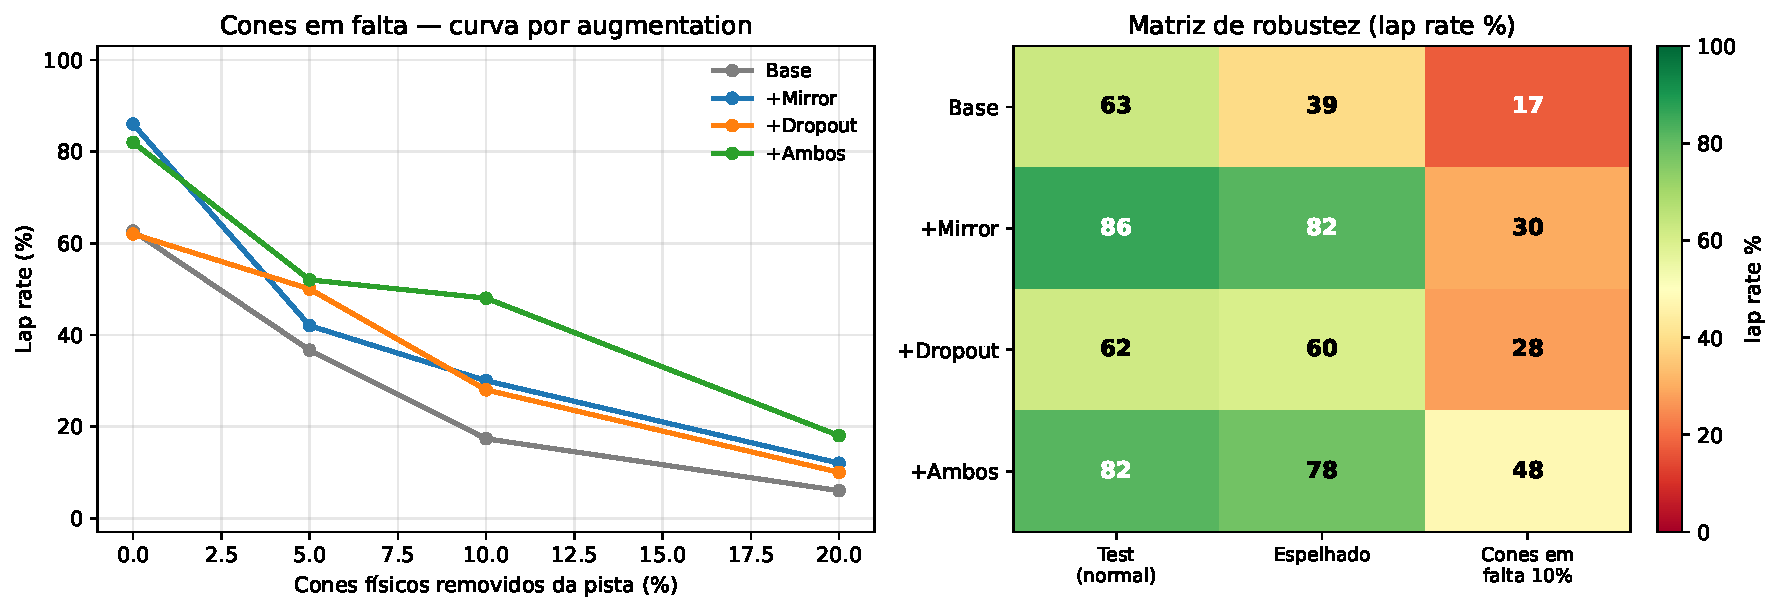
\includegraphics[width=0.88\textwidth]{figures/aug_matrix.pdf}
\caption{Robustez por \textit{augmentation}. Esquerda: \textit{lap rate} vs.\ fração de cones fisicamente removidos. Direita: matriz de robustez (\textit{lap rate} \%) dos 4 modelos do \textit{design} factorial nos três eixos de avaliação.}
\label{fig:aug_matrix}
\end{figure}

% =====================================================================
\section{Trabalho Exploratório: PacSim (sim-to-sim)}
% =====================================================================

Em paralelo, explorámos a integração com o \textbf{PacSim}, o simulador 3D em ROS\,2 usado na Formula Student, construindo uma \textit{bridge} que mapeia a perceção de cones do PacSim para o espaço de observação do agente e publica as ações como comandos de torque/\textit{steering}. A exploração validou a viabilidade do acoplamento (a política 2D produz comandos coerentes no 3D); a transferência completa fica como trabalho futuro, dependente de absorver o \textit{gap} dinâmico (\textit{pitch/roll}, \textit{slip} de pneus).

% =====================================================================
\section{Conclusões e Trabalho Futuro}
% =====================================================================

Desenvolvemos um agente de RL capaz de conduzir um carro de Formula Student \textit{Driverless} em pistas reais de competição, usando apenas a sua perceção local. As conclusões principais são: (i)~o SAC e o PPO atingem \textit{lap rates} semelhantes, mas o SAC é cerca de duas vezes mais seguro, o que o torna preferível num contexto onde cada cone é penalizado; (ii)~o SAC é marcadamente mais eficiente em amostras (3M vs.\ 6M \textit{steps}); (iii)~os \textit{splits} de teste convencionais \emph{mascaram} um viés direcional estrutural de $\sim$25\,pp, que só uma avaliação em pistas espelhadas expõe; (iv)~a robustez de perceção é assimétrica --- o \textit{flicker} transiente é tolerado, mas cones fisicamente em falta colapsam a política; e (v)~ambas as fraquezas se corrigem com \textit{data augmentation} dirigida, cuja combinação é super-aditiva e sem custo no desempenho base --- evidência de que eram limitações do protocolo de treino, não do algoritmo.

Como trabalho futuro destacam-se: a conclusão da transferência \textit{sim-to-sim} para o PacSim; a evolução para um modelo dinâmico com pneus; a avaliação multi-volta; e políticas com memória (\textit{frame-stacking}, redes recorrentes) para mitigar a observabilidade parcial --- em particular no regime de cones em falta.

% =====================================================================
\begin{thebibliography}{8}

\bibitem{kabzan2020}
Kabzan, J., et al.: AMZ Driverless: The full autonomous racing system. Journal of Field Robotics \textbf{37}(7), 1267--1294 (2020). \doi{10.1002/rob.21977}

\bibitem{sutton2018}
Sutton, R.S., Barto, A.G.: Reinforcement Learning: An Introduction. 2nd edn. MIT Press, Cambridge, MA (2018). ISBN 978-0-262-03924-6

\bibitem{kong2015}
Kong, J., Pfeiffer, M., Schildbach, G., Borrelli, F.: Kinematic and dynamic vehicle models for autonomous driving control design. In: 2015 IEEE Intelligent Vehicles Symposium (IV), pp.~1094--1099. IEEE (2015). \doi{10.1109/IVS.2015.7225830}

\bibitem{haarnoja2018}
Haarnoja, T., et al.: Soft Actor-Critic algorithms and applications. arXiv:1812.05905 (2018). \url{https://arxiv.org/abs/1812.05905}

\bibitem{schulman2017}
Schulman, J., Wolski, F., Dhariwal, P., Radford, A., Klimov, O.: Proximal Policy Optimization algorithms. arXiv:1707.06347 (2017). \url{https://arxiv.org/abs/1707.06347}

\bibitem{raffin2021}
Raffin, A., Hill, A., Gleave, A., Kanervisto, A., Ernestus, M., Dormann, N.: Stable-Baselines3: reliable reinforcement learning implementations.Journal of Machine Learning Research \textbf{22}(268), 1--8 (2021). \url{https://jmlr.org/papers/v22/20-1364.html}

\bibitem{tobin2017}
Tobin, J., Fong, R., Ray, A., Schneider, J., Zaremba, W., Abbeel, P.: Domain randomization for transferring deep neural networks from simulation to the real world. In: 2017 IEEE/RSJ IROS, pp.~23--30 (2017). \doi{10.1109/IROS.2017.8202133}

\bibitem{ulrich2024}
Ulrich, F., Wehrli, T.: End-to-End deep reinforcement learning for autonomous racing dynamics. Bachelor Thesis, ZHAW School of Engineering (2024). \url{https://doi.org/10.21256/zhaw-32000}

\end{thebibliography}

\end{document}